Genetic algorithms provide a search technique analogous to biological evolution in which instead of searching from general to specific solutions, or from more simple to complex, genetic algorithms generate solutions by mutating and combining parts of the best previously known solutions.
At each step in the search for the best solution a collection of solutions called the current \textit{population} is refined by replacing members with solutions representing the offspring of the best individuals.
The goals is then to find the best solution to the problem as determined by some criteria, called the \textit{fitness function}.
The genetic algorithm typically consist of four tasks: creating an initial population, evaluating that populations fitness, selecting members of the current population to breed, and then applying genetic operators to the selected members to breed the new population. 
This is completed until either a maximum generation is reached or the desired fitness is achieved, as shown in \autoref{alg:GAOutline}.
\begin{algorithm}
  \caption{Genetic Program Outline}
  \label{alg:GAOutline}
  \begin{algorithmic}
    \WHILE{$error>goal$}
      \FORALL{$t\in F$}
        \STATE{Compute fitness}
      \ENDFOR
      \FORALL{$t\in F$}
        \STATE{Choose individuals based on fitness}
      \ENDFOR
      \STATE{Select individuals for next population}
      \STATE{Crossover selected individuals}
      \STATE{Mutate selected individual}
    \ENDWHILE
  \end{algorithmic}
\end{algorithm}

\subsection{Problem Representation}
The thickness of the RPM  (\SI{12.7}{\cm}) was divided into slices, where each slice could be either a detector slice or a moderator slice.
These slices of detector material (represented as a \verb+1+) or moderator material (represented as a \verb+0+) were append into a sequence.
This sequence of one's and zero's (or bit string) then completely represented the geometry of the RPM and formed the basis for all possible solutions to the optimization problem.
For example the sequence \verb+0001110010+ would represent a detector that had three moderator slices, three detector slices, another two moderator slices, and a final detector slice before a single moderator slice as the reflector.
Examples of two different genomes are shown in \autoref{fig:ExGeoGenomes}
\begin{figure}

  \caption[Example Geometries Genomes]{Example of Geometry Genomes}
  \caption{fig:ExGeoGenomes}
\end{figure}
In terms of genetic algorithms the set of all possible solutions is referred to as the \textit{genome}.
The length of the genome is thus the number of slices in the geometry, where a higher length genome allows for a more complicated geometry.
The initial population for the genetic algorithm was initialized to be random bit strings with equal probability of a slice being a detector slice or moderator.

\subsection{Population Selection}
Several different selection techniques are available to select the individuals from one population to reproduce in the next.
Among the most common are fitness proportional selection (roulette selection) and tournament selection.
Roulette selection occurs when the individuals are ranked by their fitness, and individuals are chosen by their fitness rank.
This is analogous to a roulette wheel where the space a candidate occupies on the wheel is proportional to its fitness.
Higher fitness individuals will occupy more space, and will thus have a higher probability of being selected.
Tournament selection is another selection technique in which a pool of solutions are chosen at random from the current population.
Within this tournament pool a fitness proportional selection will be used to select individuals for the next generation.
The fitness function will be explained in detail in \autoref{sec:FitnessFunc}.

\subsection{Genetic Operators}
Individuals selected for reproduction are subjected to genetic operators to breed the next generation. 
Genetic programs generally contain two genetic operators, crossover and mutation. 
Crossover serves to create new members of the population by interchanging the genetic material of two parents in which significant changes in the solutions are achieved. 
Mutation serves to slightly modify an existing solution. 

Crossover is defined in genetic programming as the swapping of genetic material from one individual to another.  
For bit strings several crossover operations are commonly used; they are 1) single point crossover, 2) two point crossover, and 3) uniform crossover.
An example of the crossover operations are shown in \autoref{fig:GeneticCrossover}.
In single point crossover a single point is selected on both parents genes and the genetic material between the two parents is swapped.
In two point crossover two points are chosen on the parents bit strings and the genetic material is swapped between the intervals.
Uniform crossover uses a set mixing ratio for which according to that ratio an individual bit will be interchanged between the two parents to yield the daughters.
\begin{figure}
  \begin{subfigure}[b]{0.3\textwidth}
    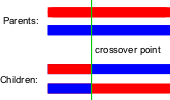
\includegraphics[width=\textwidth]{SinglePointCrossover}
    \caption{Single Point Crossover}
  \end{subfigure}
  ~
  \begin{subfigure}[b]{0.3\textwidth}
    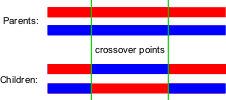
\includegraphics[width=\textwidth]{TwoPointCrossover}
    \caption{Two Point Crossover}
  \end{subfigure}
  ~
  \begin{subfigure}[b]{0.3\textwidth}
    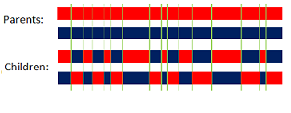
\includegraphics[width=\textwidth]{UniformCrossover}
    \caption{Uniform Crossover}
  \end{subfigure}
  \caption[Genetic Crossover Operations]{Genetic Crossover Operations. Images from Wikipedia}
  \label{fig:GeneticCrossover}
\end{figure}

Mutation is used to produce small, random changes in the genomes to maintain genetic diversity.
The mutation operation was chosen to be a simple bit flip in which a randomly chosen \verb+1+ or \verb+0+ in the geometry was flipped; for example \verb+001001010+ could be mutated to \verb+001001000+.
Generally the mutation rate is set very low (less than 2\%) in order to prevent the search for the solution to becoming simply a random search.
In this representation of the problem a mutation produces a very large change in the solution and the mutation rate was set even lower.

\subsection{Fitness Function}
\label{sec:FitnessFunc}
The fitness function defines the criteria for ranking solutions and probabilistically including them in the next generation.
The fitness function was chosen to count rate per mass of \iso[6]{Li}, provided that the geometry meet the total count rate criteria.
If it failed to meet the count rate criteria a zero fitness was returned \eqref{eqn:FitnessFun}.
\begin{align}
    \label{eqn:FitnessFun}
    f(\vec{x})
    = \begin{cases}
    0 & \text{if} \text{countRate}(\vec{x}) \leq \SI{2.5}{cps\per\nano\gram\iso[252]{Cf}} \\
    \text{countRatePerMass}(\vec{x})
    \end{cases}
\end{align}
Films that have excessive detector layers will be penalized by the normalization by the mass of \iso[6]{Li} that they contain, while favoring films that have the minimum number of detector layers that meet the count rate criteria and have a more effective utilization of the neutron flux which increase their count rate.

At this point it is instructive to make a note about the size of the solution space.
\autoref{tab:BitStringGeo} some of the these geometries are simple enough that the search space can be computed exhaustively.
\begin{table}
    \caption[Genome Bit String Geometries]{Bit String Simplified Geometry Descriptions}
    \label{tab:BitStringGeo}
    \centering
    \begin{tabular}{ c | c c}
     \toprule
     Genome Length&Slice Thickness&Possible Geometries \\
     \midrule
        5&2.54&31\\
        10&1.2700&1,023\\
        15&0.8467&32,765\\
        20&0.6350&1,048,575\\
        25&0.5080&33,554,431\\
        30&0.4233&\num{1.07E9}\\
        35&0.3629&\num{3.44E10}\\
        40&0.3175&\num{1.10E12}\\
    \bottomrule
    \end{tabular}
\end{table}
There are several salient features highlighted in \autoref{tab:BitStringGeo}.
For small genome lengths (less than 10) it is possible to exhaustively search the hypothesis space of possible solutions.
This is not possible for the larger genome lengths.
Therefore, efficient evaluation of the fitness function is necessary in order to evolve a reasonable number of solutions.
In addition the refinement in the details of the geometries increases linearly with the genome length while the size of the search space increases as $2^n$.
This suggest that a hybrid method of finding a basic geometry in a low search space and then preforming perturbations on that geometry will have a better performance than attempting to search the higher geometry solution space.
